\documentclass[addpoints,12pt]{exam}
\usepackage{amssymb}

\usepackage[pdftex]{graphicx}


\usepackage[fleqn]{amsmath}
%Forces math environment \[   MATH  \]   stuff to align much further left

\usepackage{siunitx} % Typeset SI units nicely



	\usepackage{environ}
	\NewEnviron{Answer}
	{%
	\noindent
	\rotatebox[origin=c]{180}{%
	\noindent
	\begin{minipage}[t]{\linewidth}
	\BODY
	\end{minipage}%
	}%
	}%
		% Above code grabbed from http://tex.stackexchange.com/questions/161788/how-to-have-upside-down-text-in-body . Refer back to that in the future when creating standard template for practice problem handouts.

\everymath{\displaystyle}
%All in-line math gets put in displaystyle



\headrule
%Puts a ruled line under the header on every page

\newcommand{\es}[1]{\vspace{\stretch{#1}}} 
%Even Spacing Command. Remember, you have to fill the \es{__} command's argument with a decimal number. That number determines the weight of its share of the space.

\newcommand{\as}{\vspace{1.1in}}
%A small Space: Appropriate to go after questions where 2 or 3 lines of writing will be enough.

\newcommand{\bs}{\vspace{2.5in}}
%a Big Space: Appropriate to go after questions where 4 or 5 lines of writing will be enough.

\newcommand{\cs}{\vspace{4in}}
%a Crazy big Space: Appropriate to go after questions where 7 or 8 lines of writing will be enough.

%For spaces needed that are different than above, simply use \vspace{__}, or if you want to make sure the space persists no matter what typesetting TeX thinks it should do, use \vspace*{__}.

\newcommand{\dx}{\mathrm{d}x}
%This gives a correct dx for derivatives and intergrals.

\newcommand{\dy}{\mathrm{d}y}
%This gives a correct dx for derivatives and intergrals.


\newcommand{\ts}{\textsuperscript}
%The odd case when I want to short-hand 1st, 2nd, 3rd, etc. (Useful for Newton's Laws, yaknow?)



%Header for Test
\header{Trigonometry}{www.\textbf{ChipmunkMath}.com}{Pythagorean Theorem}

\begin{document}
\begin{center}
%Title of Course goes here
\huge Practice Problems

%Title of HW goes here
\Large Pythagorean Theorem

\end{center}


\begin{center} \fbox{\fbox{\parbox{5.5in}{\centering
Difficulty level key: \quad \raisebox{-3.5pt}{\textbf{*}} $\leftrightarrow$ basic, \quad \raisebox{-3.5pt}{\textbf{**}} $\leftrightarrow$ advanced, \quad \raisebox{-3.5pt}{\textbf{***}} $\leftrightarrow$ challenge}}}
\end{center}

\vspace{0.2in}


%%%%%%%%%%%%%QUESTIONS%%%%%%%%%%%%%%%%%%%

\begin{questions}
\question
(\textbf{*})
Solve for the unknown side.

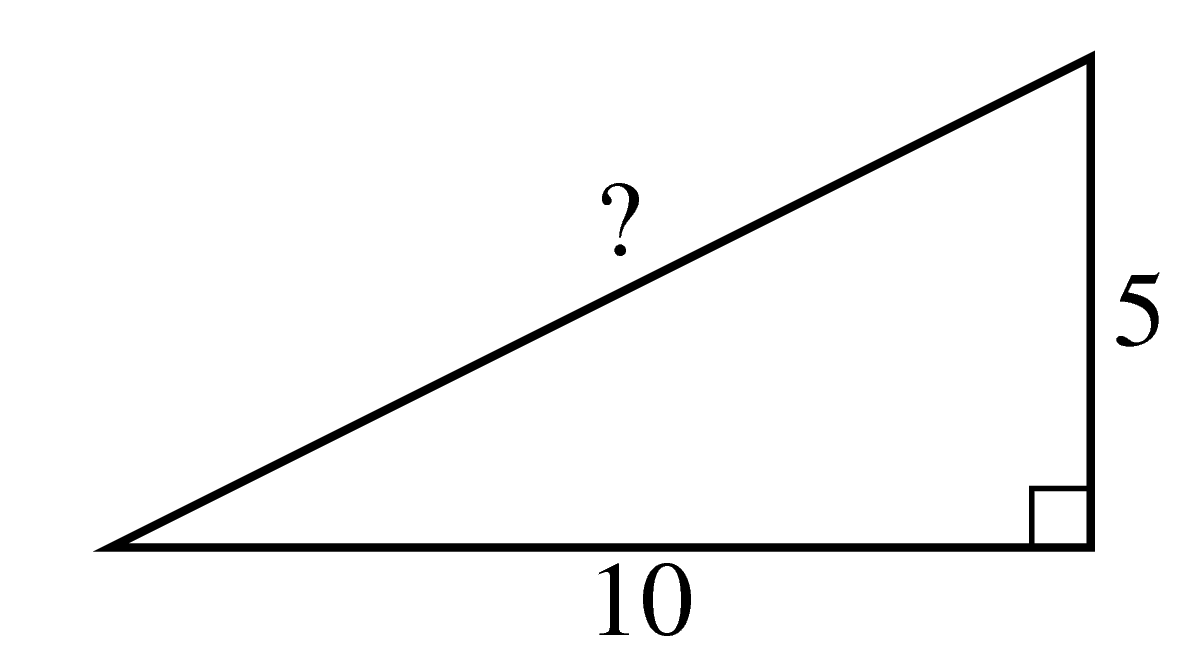
\includegraphics[width=0.4\textwidth]{../images/d1.png}

\vspace{0.3in}



%%%  

\question
(\textbf{*})
Solve for the value of $u$.

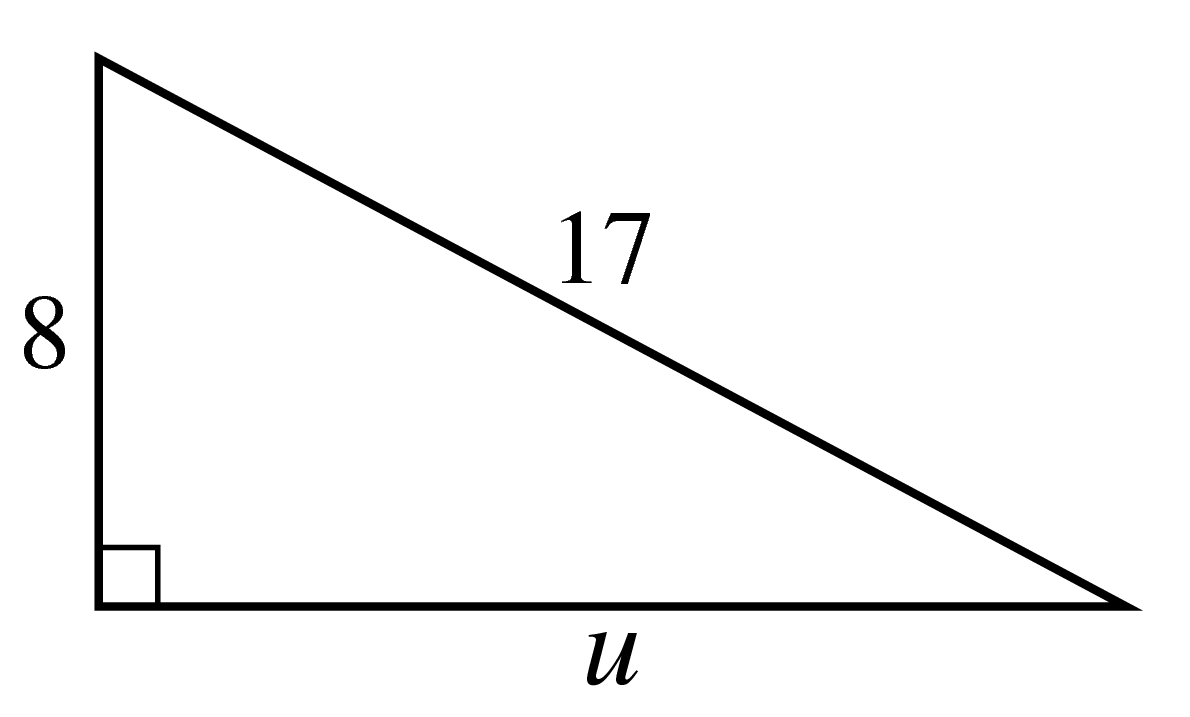
\includegraphics[width=0.4\textwidth]{../images/d3.png}

\vspace{0.3in}

%%%  

\question
(\textbf{*})
Which of the below are right triangles?

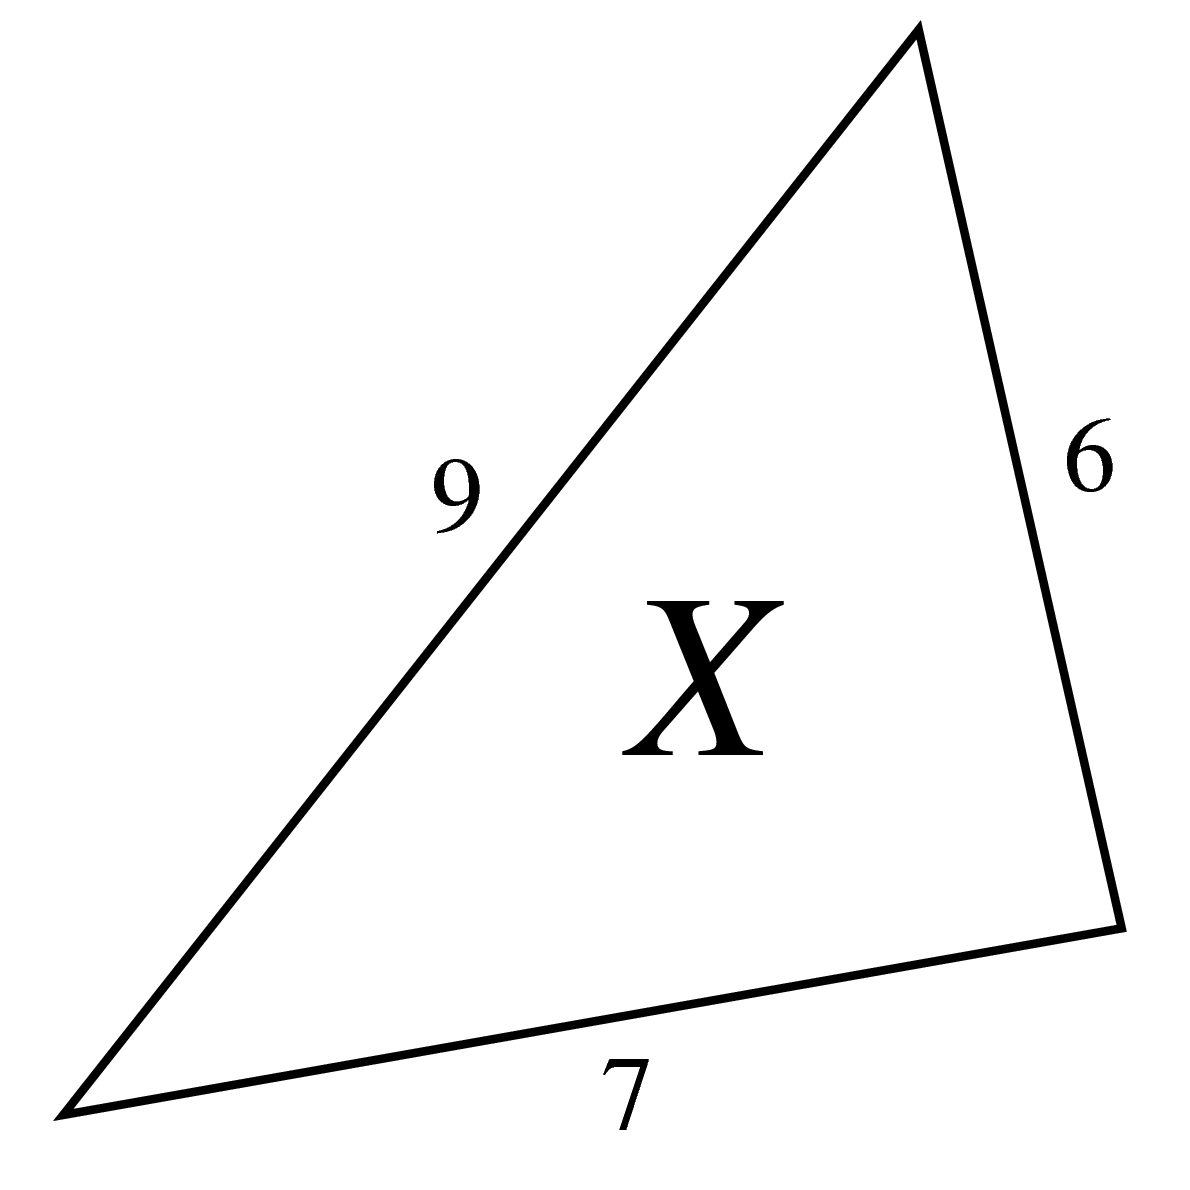
\includegraphics[width=0.4\textwidth]{../images/d4.png}
\hspace{0.2\textwidth}
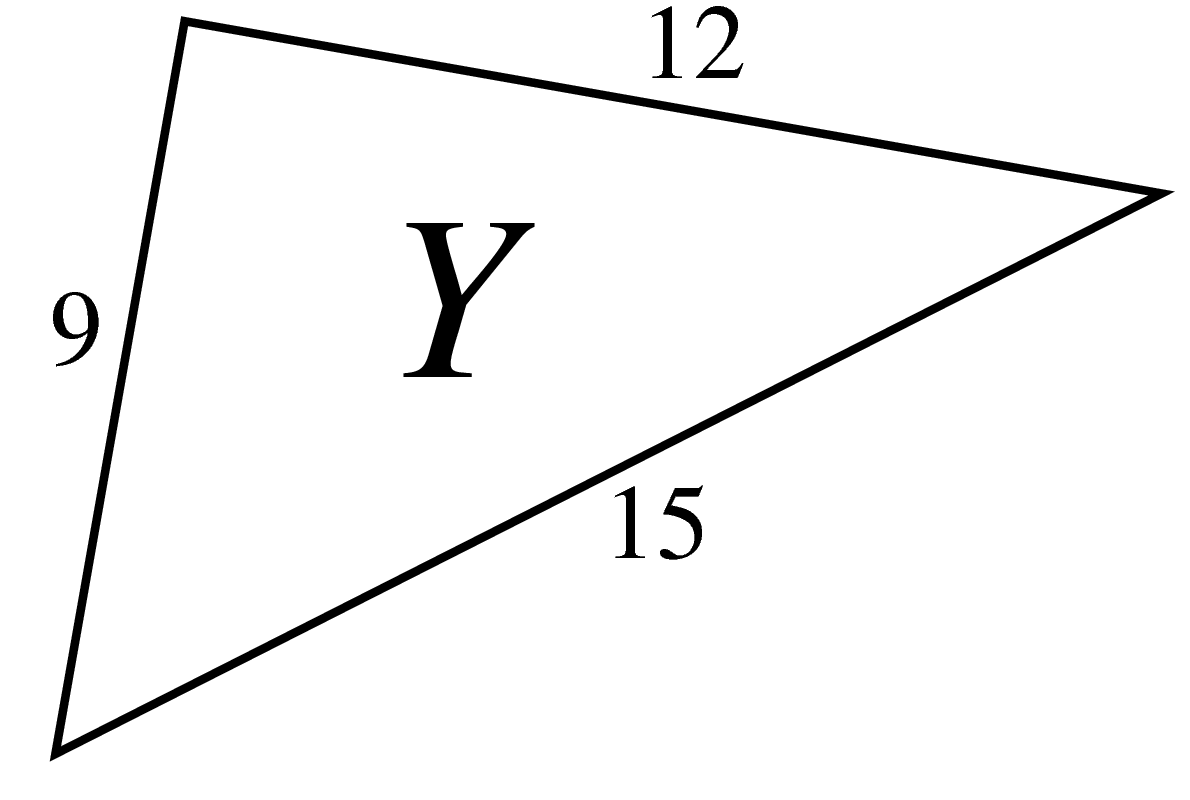
\includegraphics[width=0.4\textwidth]{../images/d5.png}

\vspace{0.2in}


%%%
\newpage


\question
(\textbf{**})
Solve for $x$.

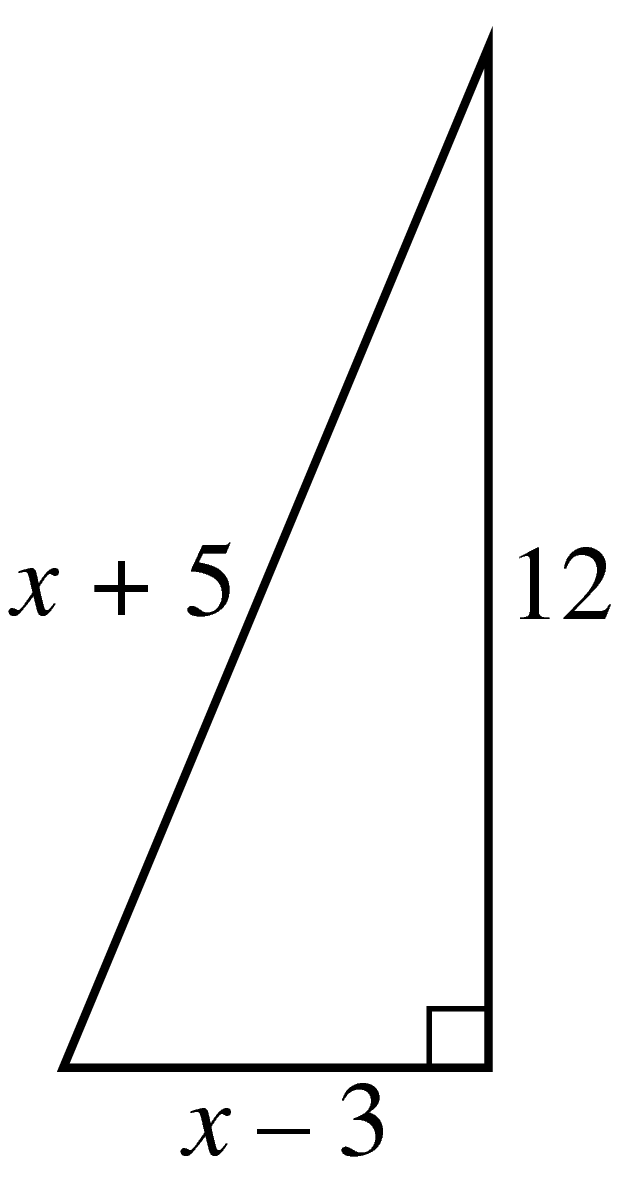
\includegraphics[width=0.2\textwidth]{../images/d6.png}

\vspace{0.3in}

%%%  

\question
(\textbf{**})
How long is the square's diagonal?

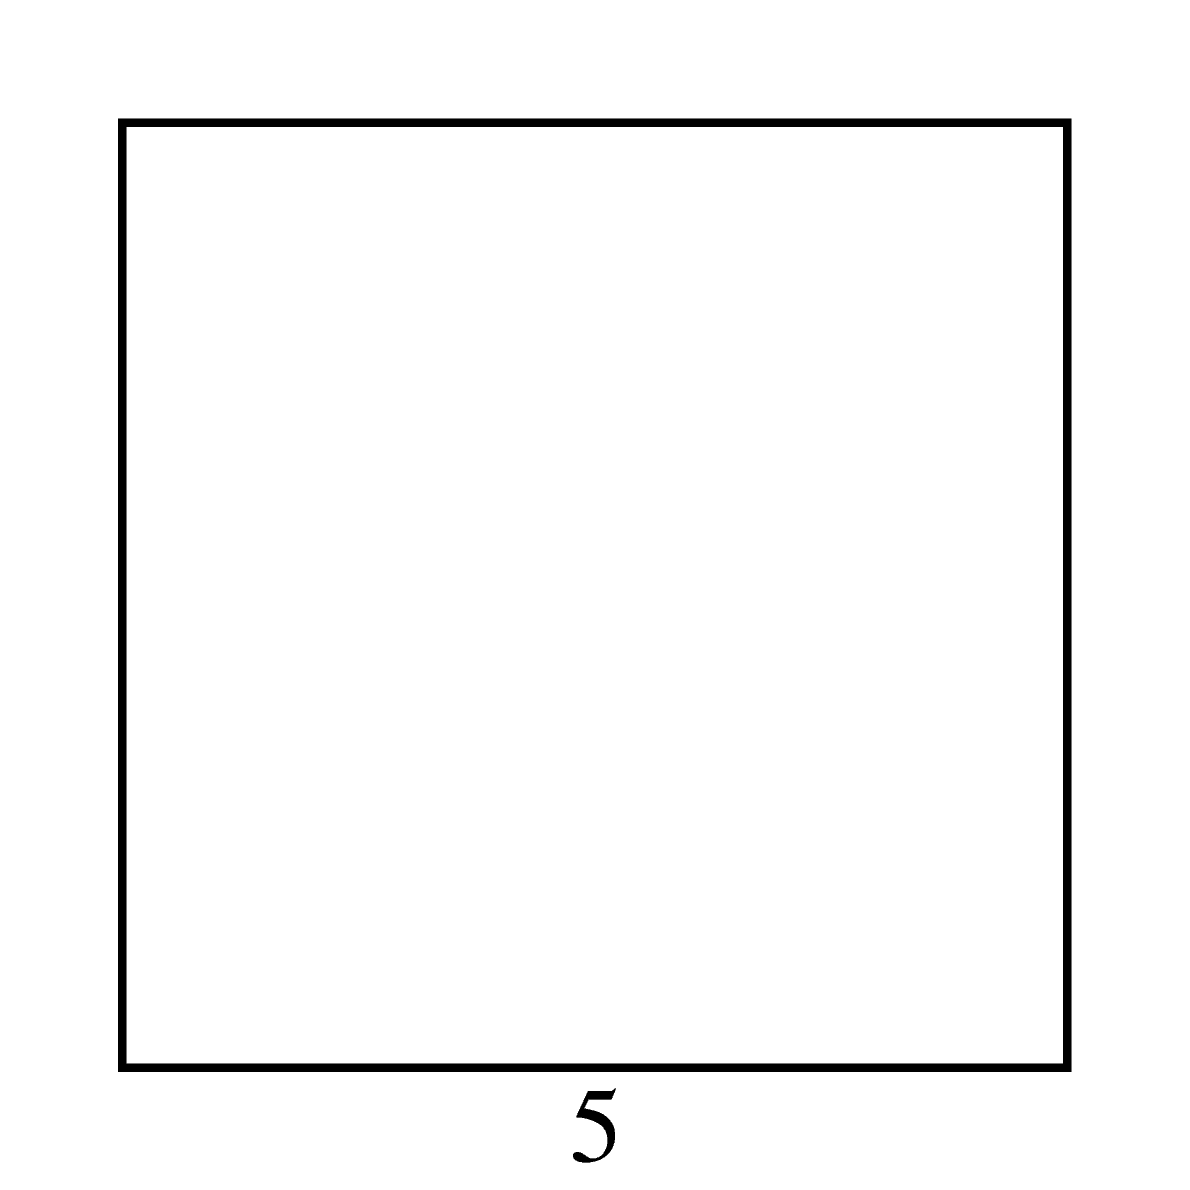
\includegraphics[width=0.4\textwidth]{../images/d8.png}

\vspace{0.3in}

%%%  

\question
(\textbf{***})
Tom is painting a building. He has a ladder that's $4\si{\m}$ long. To do the painting, the top of the ladder must be at least $3.5 \si{\m}$ up the wall. What is the farthest that the bottom of the ladder can be from the wall?
\vspace{0.3in}

%%%  END OF QUESTIONS %%%

\vfill % Fills to bottom so that answerbox is typeset at end of page.


\begin{Answer}
	\fbox{\textbf{Answers:} 
	1. $5\sqrt{5}$, \quad
	2. 15, \quad
	3. $X$ is not, $Y$ is, \quad
	4. 8, \quad
	5. $5\sqrt{2}$, \quad
	6. $1.94 \si{\m}$
	  }
\end{Answer}



\end{questions}
\end{document}